\documentclass[12pt,a4paper]{article}

% Sử dụng chuẩn font mặc định của LaTeX (Computer Modern) và hỗ trợ Tiếng Việt
\usepackage[T5]{fontenc}
\usepackage[utf8]{inputenc}

\usepackage{amsmath}
\usepackage{amsfonts}
\usepackage{amssymb}
\usepackage{graphicx}
\usepackage[margin=2cm]{geometry}
\usepackage{tikz}
\usepackage{circuitikz}
\usepackage{listings}
\usepackage{xcolor}
\usepackage{hyperref}

% Cấu hình hiển thị code Verilog, TCL, Python
\lstdefinestyle{verilogstyle}{
    language=Verilog,
    basicstyle=\ttfamily\footnotesize,
    keywordstyle=\color{blue},
    commentstyle=\color{green!60!black},
    stringstyle=\color{red},
    numbers=left,
    numberstyle=\tiny\color{gray},
    stepnumber=1,
    numbersep=10pt,
    backgroundcolor=\color{gray!5},
    frame=single,
    rulecolor=\color{black!30},
    breaklines=true,
    breakatwhitespace=true,
    tabsize=4,
    showstringspaces=false
}

\lstdefinestyle{tclstyle}{
    language=tcl,
    basicstyle=\ttfamily\footnotesize,
    keywordstyle=\color{blue},
    commentstyle=\color{green!60!black},
    stringstyle=\color{red},
    numbers=left,
    numberstyle=\tiny\color{gray},
    stepnumber=1,
    numbersep=10pt,
    backgroundcolor=\color{gray!5},
    frame=single,
    rulecolor=\color{black!30},
    breaklines=true,
    tabsize=4
}

\title{\textbf{GIẢI CHI TIẾT ĐỀ THI CUỐI KỲ}\\MÔN: THIẾT KẾ ASIC VÀ LÕI IP (Năm 2012-2013)}
\author{Biên soạn bởi: AI System}
\date{\today}

\begin{document}

\maketitle
\tableofcontents
\newpage

% ==============================================================================
\section{Bài 1 (1.5đ): Áp dụng Coding Guideline}
\textbf{ĐỀ BÀI:} \\
a) Hãy áp dụng Coding Guideline cho thiết kế IP vào đoạn code Verilog sau:\\
b) Hãy liệt kê các Guideline đã áp dụng được.

\textit{Code chưa áp dụng Guideline:}
\begin{lstlisting}[style=verilogstyle]
module LCD_Controller (  
//Host Side 
iDATA,iRS, 
Start,oDone, 
CLK,RST_N, 
//LCD Interface 
LCD_DATA, 
LCD_RW, 
LCD_EN, 
LCD_RS); 
...
\end{lstlisting}

\hrule\vspace{0.5cm}
\textbf{LỜI GIẢI:}

\textbf{a) Code áp dụng Guideline}

\begin{lstlisting}[style=verilogstyle]
`timescale 1ns / 1ps

module LCD_Controller (
    // Clock and Reset
    input  wire       CLK,
    input  wire       RST_N,
    
    // Host Side Interfaces
    input  wire [7:0] iDATA,
    input  wire       iRS,
    input  wire       Start,
    output reg        oDone,
    
    // LCD Interfaces
    output wire [7:0] LCD_DATA,
    output wire       LCD_RW,
    output reg        LCD_EN,
    output wire       LCD_RS
);

    // ==========================================
    // Internal Registers and Wires
    // ==========================================
    reg [4:0] Cont_r;        // Counter register
    reg [1:0] ST_r;          // State machine register
    reg       preStart_r;    // Previous start signal
    reg       mStart_r;      // Start pulse detection

    // ==========================================
    // Continuous Assignments
    // ==========================================
    assign LCD_DATA = iDATA;
    assign LCD_RW   = 1'b0;  // Write only mode
    assign LCD_RS   = iRS;   // Bypass iRS to LCD_RS

    // ==========================================
    // Sequential Logic
    // ==========================================
    always @(posedge CLK or negedge RST_N) begin
        if (!RST_N) begin
            // Reset state
            oDone      <= 1'b0;
            LCD_EN     <= 1'b0;
            preStart_r <= 1'b0;
            mStart_r   <= 1'b0;
            Cont_r     <= 5'b00000;
            ST_r       <= 2'b00;
        end else begin
            // Edge detection for Start signal
            preStart_r <= Start;
            
            if ({preStart_r, Start} == 2'b01) begin
                mStart_r <= 1'b1;
                oDone    <= 1'b0;
            end
            
            // State Machine execution
            if (mStart_r) begin
                case (ST_r)
                    2'b00: begin // State 0
                        ST_r <= 2'b01;
                    end
                    
                    2'b01: begin // State 1: Wait Setup
                        LCD_EN <= 1'b1;
                        ST_r   <= 2'b10;
                    end
                    
                    2'b10: begin // State 2: Clock divide
                        if (Cont_r < 5'd16) begin
                            Cont_r <= Cont_r + 5'd1;
                        end else begin
                            ST_r <= 2'b11;
                        end
                    end
                    
                    2'b11: begin // State 3: Done
                        LCD_EN   <= 1'b0;
                        mStart_r <= 1'b0;
                        oDone    <= 1'b1;
                        Cont_r   <= 5'b00000;
                        ST_r     <= 2'b00;
                    end
                    
                    default: begin // Safe State Machine fallback
                        ST_r <= 2'b00;
                    end
                endcase
            end
        end
    end

endmodule
\end{lstlisting}

\textbf{b) Liệt kê các Guideline đã áp dụng:}
\begin{enumerate}
    \item \textbf{Cấu trúc file (File Header \& Timescale):} Bổ sung chỉ thị `timescale.
    \item \textbf{Khai báo I/O theo chuẩn ANSI C/Verilog-2001:} Tích hợp trực tiếp hướng (\texttt{input/output}), loại tín hiệu (\texttt{wire/reg}) và độ rộng bit vào chung danh sách tham số của module giúp code gọn gàng, tránh khai báo thừa hoặc lỗi thiếu sót.
    \item \textbf{Thụt lề (Indentation \& Alignment):} Căn lề code đúng chuẩn (Tab size = 4 spaces). Căn thẳng hàng tên biến, kiểu dữ liệu và ký hiệu gán.
    \item \textbf{Quy ước đặt tên (Naming Convention):} Thêm hậu tố \texttt{\_r} cho các thanh ghi nội bộ (vd: \texttt{Cont\_r}, \texttt{ST\_r}, \texttt{mStart\_r}) để phân biệt rõ ràng với port giao tiếp.
    \item \textbf{Cấu trúc khối (Block Structure):} Sử dụng \texttt{begin} / \texttt{end} cho mọi cấu trúc điều kiện (\texttt{if-else}) và \texttt{case}, kể cả khi chỉ có 1 lệnh.
    \item \textbf{Mô tả FSM an toàn (Safe State Machine):} Cung cấp giá trị \texttt{default} trong khối \texttt{case} để đảm bảo FSM không bị kẹt ở trạng thái không xác định (latch phòng ngừa).
    \item \textbf{Định nghĩa độ rộng bit rõ ràng (Explicit bit width):} Đổi \texttt{16} thành \texttt{5'd16}, \texttt{0} thành \texttt{5'b00000} (với Cont\_r) và \texttt{2'b00} (với ST\_r) để không phụ thuộc vào độ rộng default (32-bit integer).
\end{enumerate}


% ==============================================================================
\section{Bài 2 (2đ): Vẽ Stick Diagram công nghệ CMOS}
\textbf{ĐỀ BÀI:} \\
Hãy vẽ các cổng logic sau bằng stick diagram sử dụng công nghệ CMOS\\
- 4-input NAND\\
- 4-input NOR\\
- 3-input AND\\
- 3-input OR

\hrule\vspace{0.5cm}
\textbf{LỜI GIẢI:}

Stick diagram CMOS mô tả sắp xếp các dải khuyếch tán (diffusion) P+ và N+, các dải Polysilicon (cổng Gate), và kim loại (Metal) nối VDD/GND.

\begin{itemize}
    \item \textbf{4-input NAND:} Mạng PDN (N-MOS) gồm 4 transistor mắc \textbf{nối tiếp}. Mạng PUN (P-MOS) gồm 4 transistor mắc \textbf{song song}.
    \item \textbf{4-input NOR:} Mạng PUN (P-MOS) gồm 4 transistor mắc \textbf{nối tiếp}. Mạng PDN (N-MOS) gồm 4 transistor mắc \textbf{song song}.
    \item \textbf{3-input AND:} Là cổng 3-input NAND nối tiếp với 1 cổng NOT (Inverter).
    \item \textbf{3-input OR:} Là cổng 3-input NOR nối tiếp với 1 cổng NOT (Inverter).
\end{itemize}

\begin{figure}[h!]
    \centering
    % NAND4
    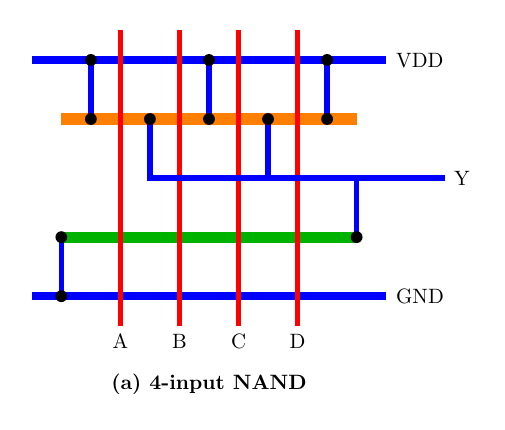
\begin{tikzpicture}[scale=0.75, transform shape]
        \draw[blue, line width=3pt] (0, 4) -- (6, 4) node[right, black] {VDD};
        \draw[blue, line width=3pt] (0, 0) -- (6, 0) node[right, black] {GND};
        \draw[orange, line width=4pt] (0.5, 3) -- (5.5, 3);
        \draw[green!70!black, line width=4pt] (0.5, 1) -- (5.5, 1);
        \draw[red, line width=2pt] (1.5, -0.5) node[below, black] {A} -- (1.5, 4.5);
        \draw[red, line width=2pt] (2.5, -0.5) node[below, black] {B} -- (2.5, 4.5);
        \draw[red, line width=2pt] (3.5, -0.5) node[below, black] {C} -- (3.5, 4.5);
        \draw[red, line width=2pt] (4.5, -0.5) node[below, black] {D} -- (4.5, 4.5);
        % PUN
        \draw[blue, line width=2pt] (1, 4) -- (1, 3); \fill[black] (1, 4) circle (0.1); \fill[black] (1, 3) circle (0.1);
        \draw[blue, line width=2pt] (3, 4) -- (3, 3); \fill[black] (3, 4) circle (0.1); \fill[black] (3, 3) circle (0.1);
        \draw[blue, line width=2pt] (5, 4) -- (5, 3); \fill[black] (5, 4) circle (0.1); \fill[black] (5, 3) circle (0.1);
        \draw[blue, line width=2pt] (2, 3) -- (2, 2) -- (4, 2) -- (4, 3); 
        \fill[black] (2, 3) circle (0.1); \fill[black] (4, 3) circle (0.1);
        % PDN
        \draw[blue, line width=2pt] (5.5, 1) -- (5.5, 2) -- (4, 2); \fill[black] (5.5, 1) circle (0.1);
        \draw[blue, line width=2pt] (4, 2) -- (7, 2) node[right, black] {Y};
        \draw[blue, line width=2pt] (0.5, 1) -- (0.5, 0); \fill[black] (0.5, 1) circle (0.1); \fill[black] (0.5, 0) circle (0.1);
        \node at (3, -1.5) {\textbf{(a) 4-input NAND}};
    \end{tikzpicture}
    \hspace{0.5cm}
    % NOR4
    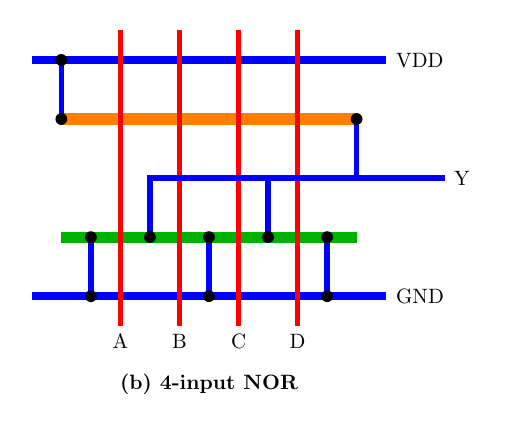
\begin{tikzpicture}[scale=0.75, transform shape]
        \draw[blue, line width=3pt] (0, 4) -- (6, 4) node[right, black] {VDD};
        \draw[blue, line width=3pt] (0, 0) -- (6, 0) node[right, black] {GND};
        \draw[orange, line width=4pt] (0.5, 3) -- (5.5, 3);
        \draw[green!70!black, line width=4pt] (0.5, 1) -- (5.5, 1);
        \draw[red, line width=2pt] (1.5, -0.5) node[below, black] {A} -- (1.5, 4.5);
        \draw[red, line width=2pt] (2.5, -0.5) node[below, black] {B} -- (2.5, 4.5);
        \draw[red, line width=2pt] (3.5, -0.5) node[below, black] {C} -- (3.5, 4.5);
        \draw[red, line width=2pt] (4.5, -0.5) node[below, black] {D} -- (4.5, 4.5);
        % PUN
        \draw[blue, line width=2pt] (0.5, 4) -- (0.5, 3); \fill[black] (0.5, 4) circle (0.1); \fill[black] (0.5, 3) circle (0.1);
        \draw[blue, line width=2pt] (5.5, 3) -- (5.5, 2); \fill[black] (5.5, 3) circle (0.1);
        % PDN
        \draw[blue, line width=2pt] (1, 0) -- (1, 1); \fill[black] (1, 0) circle (0.1); \fill[black] (1, 1) circle (0.1);
        \draw[blue, line width=2pt] (3, 0) -- (3, 1); \fill[black] (3, 0) circle (0.1); \fill[black] (3, 1) circle (0.1);
        \draw[blue, line width=2pt] (5, 0) -- (5, 1); \fill[black] (5, 0) circle (0.1); \fill[black] (5, 1) circle (0.1);
        \draw[blue, line width=2pt] (2, 1) -- (2, 2) -- (4, 2) -- (4, 1); 
        \fill[black] (2, 1) circle (0.1); \fill[black] (4, 1) circle (0.1);
        \draw[blue, line width=2pt] (4, 2) -- (5.5, 2) -- (7, 2) node[right, black] {Y};
        \node at (3, -1.5) {\textbf{(b) 4-input NOR}};
    \end{tikzpicture}
    
    \vspace{0.8cm}
    % AND3 (NAND3 + NOT)
    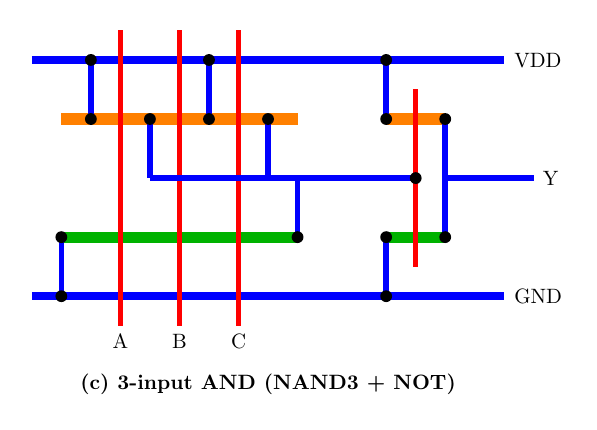
\begin{tikzpicture}[scale=0.75, transform shape]
        \draw[blue, line width=3pt] (0, 4) -- (8, 4) node[right, black] {VDD};
        \draw[blue, line width=3pt] (0, 0) -- (8, 0) node[right, black] {GND};
        \draw[orange, line width=4pt] (0.5, 3) -- (4.5, 3);
        \draw[green!70!black, line width=4pt] (0.5, 1) -- (4.5, 1);
        \draw[red, line width=2pt] (1.5, -0.5) node[below, black] {A} -- (1.5, 4.5);
        \draw[red, line width=2pt] (2.5, -0.5) node[below, black] {B} -- (2.5, 4.5);
        \draw[red, line width=2pt] (3.5, -0.5) node[below, black] {C} -- (3.5, 4.5);
        \draw[blue, line width=2pt] (1, 4) -- (1, 3); \fill[black] (1, 4) circle (0.1); \fill[black] (1, 3) circle (0.1);
        \draw[blue, line width=2pt] (3, 4) -- (3, 3); \fill[black] (3, 4) circle (0.1); \fill[black] (3, 3) circle (0.1);
        \draw[blue, line width=2pt] (2, 3) -- (2, 2); \fill[black] (2, 3) circle (0.1);
        \draw[blue, line width=2pt] (4, 3) -- (4, 2) -- (2, 2); \fill[black] (4, 3) circle (0.1);
        \draw[blue, line width=2pt] (4.5, 1) -- (4.5, 2) -- (4, 2); \fill[black] (4.5, 1) circle (0.1);
        \draw[blue, line width=2pt] (0.5, 1) -- (0.5, 0); \fill[black] (0.5, 1) circle (0.1); \fill[black] (0.5, 0) circle (0.1);
        \draw[orange, line width=4pt] (6, 3) -- (7, 3);
        \draw[green!70!black, line width=4pt] (6, 1) -- (7, 1);
        \draw[red, line width=2pt] (6.5, 0.5) -- (6.5, 3.5);
        \draw[blue, line width=2pt] (4, 2) -- (6.5, 2); \fill[black] (6.5, 2) circle (0.1);
        \draw[blue, line width=2pt] (6, 4) -- (6, 3); \fill[black] (6, 4) circle (0.1); \fill[black] (6, 3) circle (0.1);
        \draw[blue, line width=2pt] (6, 1) -- (6, 0); \fill[black] (6, 1) circle (0.1); \fill[black] (6, 0) circle (0.1);
        \draw[blue, line width=2pt] (7, 3) -- (7, 1); \fill[black] (7, 3) circle (0.1); \fill[black] (7, 1) circle (0.1);
        \draw[blue, line width=2pt] (7, 2) -- (8.5, 2) node[right, black] {Y};
        \node at (4, -1.5) {\textbf{(c) 3-input AND (NAND3 + NOT)}};
    \end{tikzpicture}
    \hspace{0.5cm}
    % OR3 (NOR3 + NOT)
    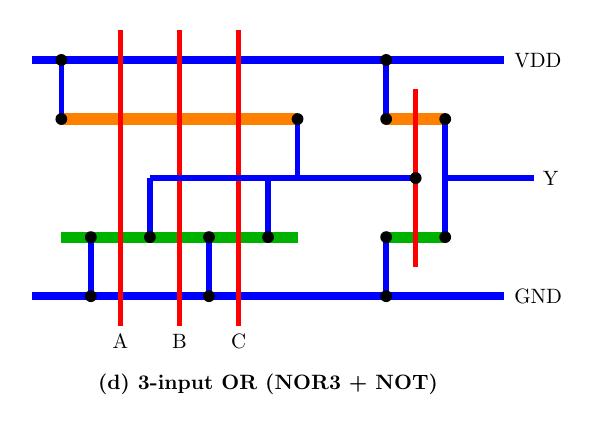
\begin{tikzpicture}[scale=0.75, transform shape]
        \draw[blue, line width=3pt] (0, 4) -- (8, 4) node[right, black] {VDD};
        \draw[blue, line width=3pt] (0, 0) -- (8, 0) node[right, black] {GND};
        \draw[orange, line width=4pt] (0.5, 3) -- (4.5, 3);
        \draw[green!70!black, line width=4pt] (0.5, 1) -- (4.5, 1);
        \draw[red, line width=2pt] (1.5, -0.5) node[below, black] {A} -- (1.5, 4.5);
        \draw[red, line width=2pt] (2.5, -0.5) node[below, black] {B} -- (2.5, 4.5);
        \draw[red, line width=2pt] (3.5, -0.5) node[below, black] {C} -- (3.5, 4.5);
        \draw[blue, line width=2pt] (0.5, 4) -- (0.5, 3); \fill[black] (0.5, 4) circle (0.1); \fill[black] (0.5, 3) circle (0.1);
        \draw[blue, line width=2pt] (4.5, 3) -- (4.5, 2); \fill[black] (4.5, 3) circle (0.1);
        \draw[blue, line width=2pt] (1, 0) -- (1, 1); \fill[black] (1, 0) circle (0.1); \fill[black] (1, 1) circle (0.1);
        \draw[blue, line width=2pt] (3, 0) -- (3, 1); \fill[black] (3, 0) circle (0.1); \fill[black] (3, 1) circle (0.1);
        \draw[blue, line width=2pt] (2, 1) -- (2, 2); \fill[black] (2, 1) circle (0.1);
        \draw[blue, line width=2pt] (4, 1) -- (4, 2) -- (2, 2); \fill[black] (4, 1) circle (0.1);
        \draw[blue, line width=2pt] (4, 2) -- (4.5, 2);
        \draw[orange, line width=4pt] (6, 3) -- (7, 3);
        \draw[green!70!black, line width=4pt] (6, 1) -- (7, 1);
        \draw[red, line width=2pt] (6.5, 0.5) -- (6.5, 3.5);
        \draw[blue, line width=2pt] (4.5, 2) -- (6.5, 2); \fill[black] (6.5, 2) circle (0.1);
        \draw[blue, line width=2pt] (6, 4) -- (6, 3); \fill[black] (6, 4) circle (0.1); \fill[black] (6, 3) circle (0.1);
        \draw[blue, line width=2pt] (6, 1) -- (6, 0); \fill[black] (6, 1) circle (0.1); \fill[black] (6, 0) circle (0.1);
        \draw[blue, line width=2pt] (7, 3) -- (7, 1); \fill[black] (7, 3) circle (0.1); \fill[black] (7, 1) circle (0.1);
        \draw[blue, line width=2pt] (7, 2) -- (8.5, 2) node[right, black] {Y};
        \node at (4, -1.5) {\textbf{(d) 3-input OR (NOR3 + NOT)}};
    \end{tikzpicture}
\end{figure}

% ==============================================================================
\section{Bài 3 (1đ): Layout cổng NOR 3 ngõ vào}
\textbf{ĐỀ BÀI:} \\
a) Hãy vẽ layout cổng NOR 3 ngõ vào, và ghi chú kích thước các bề dày của wires\\
b) Cho biết diện tích của cổng NOR 3 ngõ vào\\
(Chú ý: khoảng cách các chấm là bằng $1\lambda$)

\hrule\vspace{0.5cm}
\textbf{LỜI GIẢI:}

\textbf{a) Vẽ Layout và kích thước:}
\begin{itemize}
    \item Bề dày tối thiểu của dải Poly (Gate): $2\lambda$.
    \item Bề dày tối thiểu của Diffusion (N+ và P+): $3\lambda$ hoặc $4\lambda$ tùy rule.
    \item Bề dày tối thiểu của Metal 1 (VDD, GND): $3\lambda$ hoặc $4\lambda$.
    \item Khoảng cách Contact (Via): Kích thước lỗ $2\lambda \times 2\lambda$.
\end{itemize}

\textbf{b) Tính diện tích NOR 3:}
Phụ thuộc vào Design Rule (Lambda based rules - SCMOS). 
Một cách ước lượng cơ bản dựa vào Pitch định tuyến:
Chiều cao cell thường cố định (VD: $40\lambda$).
Chiều ngang cell phụ thuộc số đường Poly đứng: NOR 3 có 3 poly + 2 vùng contact hai bên $\approx 5$ đến 6 grid. Mỗi grid pitch tầm $8\lambda \rightarrow$ Chiều rộng $\approx 40\lambda - 48\lambda$.
Diện tích tổng (Area) = Chiều cao $\times$ Chiều rộng $\approx 40\lambda \times 40\lambda = 1600 \lambda^2$. 
\begin{figure}[h!]
    \centering
    \begin{tikzpicture}[scale=0.6, transform shape]
        % Draw grid
        \draw[step=1, gray!30, very thin] (0,0) grid (18,12);
        
        % N-well (dashed outline)
        \draw[dashed, thick] (0.5, 5.5) rectangle (17.5, 11.5) node[above left] {N-Well};
        
        % VDD and GND (Metal 1 - Blue)
        \fill[blue!50] (0, 10) rectangle (18, 11) node[midway, black] {\textbf{VDD} ($4\lambda$)};
        \fill[blue!50] (0, 0) rectangle (18, 1) node[midway, black] {\textbf{GND} ($4\lambda$)};
        
        % P+ Diffusion (Orange) inside N-Well
        \fill[orange!80] (2, 7) rectangle (15, 9);
        
        % N+ Diffusion (Green) outside N-Well
        \fill[green!70!black, opacity=0.8] (2, 2) rectangle (15, 4);
        
        % Poly (Red)
        \fill[red!80] (4, 1.5) rectangle (5, 9.5); \node[above] at (4.5, 9.5) {\textbf{A} ($2\lambda$)};
        \fill[red!80] (8, 1.5) rectangle (9, 9.5); \node[above] at (8.5, 9.5) {\textbf{B} ($2\lambda$)};
        \fill[red!80] (12, 1.5) rectangle (13, 9.5); \node[above] at (12.5, 9.5) {\textbf{C} ($2\lambda$)};
        
        % Contacts
        \fill[black] (3, 10.5) circle (0.3); \fill[black] (3, 8) circle (0.3);
        \draw[blue, line width=4pt] (3, 10.5) -- (3, 8);
        
        \fill[black] (14, 8) circle (0.3); \fill[black] (14, 3) circle (0.3);
        \draw[blue, line width=4pt] (14, 8) -- (14, 3);
        
        \draw[blue, line width=4pt] (14, 5.5) -- (17, 5.5) node[right, black] {\textbf{Output Y}};
        
        \node at (9, -1.5) {\textbf{Minh họa Layout chuẩn Lambda cho cổng NOR 3}};
    \end{tikzpicture}
\end{figure}

% ==============================================================================
\section{Bài 4 (1đ): Vẽ sơ đồ Transistor-level}
\textbf{ĐỀ BÀI:} \\
Vẽ sơ đồ transistor-level sử dụng cổng logic CMOS cho các hàm sau:\\
a) $Y = \overline{(A + B) \cdot (C + D)}$\\
b) $Y = \overline{A \cdot (B \cdot C + D)}$

\hrule\vspace{0.5cm}
\textbf{LỜI GIẢI:}

Quy tắc CMOS: Phép "Cộng" (OR) $\rightarrow$ N-MOS mắc song song, P-MOS mắc nối tiếp. Phép "Nhân" (AND) $\rightarrow$ N-MOS mắc nối tiếp, P-MOS mắc song song.

\textbf{Câu a: $Y = \overline{(A + B) \cdot (C + D)}$ (Cổng AOI22)}
\begin{figure}[h!]
    \centering
    \begin{circuitikz}[scale=0.8, transform shape]
        \draw (3, 6) node[vcc] {VDD};
        % nodes
        \node[pmos] (pA) at (1.5, 4) {A};
        \node[pmos] (pB) at (1.5, 2) {B};
        \node[pmos] (pC) at (4.5, 4) {C};
        \node[pmos] (pD) at (4.5, 2) {D};
        
        \node[nmos] (nA) at (1.5, -1) {A};
        \node[nmos] (nB) at (4.5, -1) {B};
        \node[nmos] (nC) at (1.5, -3) {C};
        \node[nmos] (nD) at (4.5, -3) {D};
        
        % connections PUN
        \draw (3,6) -- (3,5) -- (1.5,5) -- (pA.S);
        \draw (3,5) -- (4.5,5) -- (pC.S);
        \draw (pA.D) -- (pB.S);
        \draw (pC.D) -- (pD.S);
        \draw (pB.D) -- (1.5, 1) -- (4.5, 1) -- (pD.D);
        \draw (3, 1) -- (3, 0.5) node[right] {Y};
        
        % connections PDN
        \draw (3, 0.5) -- (3, 0) -- (1.5, 0) -- (nA.D);
        \draw (3, 0) -- (4.5, 0) -- (nB.D);
        \draw (nA.S) -- (1.5, -2) -- (4.5, -2) -- (nB.S);
        \draw (3, -2) -- (3, -2.5) -- (1.5, -2.5);
        \draw (3, -2.5) -- (4.5, -2.5);
        \draw (1.5, -2.5) -- (nC.D);
        \draw (4.5, -2.5) -- (nD.D);
        \draw (nC.S) -- (1.5, -4) -- (4.5, -4) -- (nD.S);
        \draw (3, -4) node[ground] {};
    \end{circuitikz}
\end{figure}

\textbf{Câu b: $Y = \overline{A \cdot (B \cdot C + D)}$}
\begin{figure}[h!]
    \centering
    \begin{circuitikz}[scale=0.8, transform shape]
        \draw (2.5, 6) node[vcc] {VDD};
        
        \node[pmos] (pA) at (1, 3) {A};
        \node[pmos] (pB) at (4, 4) {B};
        \node[pmos] (pC) at (5.5, 4) {C};
        \node[pmos] (pD) at (4.75, 2) {D};
        
        \node[nmos] (nA) at (2.5, 0) {A};
        \node[nmos] (nB) at (4, -2) {B};
        \node[nmos] (nC) at (4, -4) {C};
        \node[nmos] (nD) at (1, -3) {D};
        
        % PUN
        \draw (2.5, 6) -- (2.5, 5);
        \draw (1, 5) -- (5.5, 5);
        \draw (1, 5) -- (pA.S);
        \draw (4, 5) -- (pB.S);
        \draw (5.5, 5) -- (pC.S);
        \draw (pB.D) -- (4, 3) -- (5.5, 3) -- (pC.D);
        \draw (4.75, 3) -- (pD.S);
        \draw (pA.D) -- (1, 1) -- (4.75, 1) -- (pD.D);
        \draw (2.5, 1) -- (2.5, 0.5) node[right] {Y};
        
        % PDN
        \draw (2.5, 0.5) -- (nA.D);
        \draw (nA.S) -- (2.5, -1) -- (1, -1) -- (nD.D);
        \draw (2.5, -1) -- (4, -1) -- (nB.D);
        \draw (nB.S) -- (nC.D);
        \draw (nD.S) -- (1, -5) -- (4, -5) -- (nC.S);
        \draw (2.5, -5) node[ground] {};
    \end{circuitikz}
\end{figure}

% ==============================================================================
\section{Bài 5 (1.5đ): Synopsys Design Compiler constraints}
\textbf{ĐỀ BÀI:} \\
Cho sơ đồ thiết kế (xem hình)\\
a) Viết script cho Synopsys Design Compiler có tên là “my\_constraints” để tạo các constraints sau:\\
- Maximum operating clock 150MHz\\
- Clock latency 1ns\\
- Clk\_en delay 1ns\\
- Reset delay 1ns\\
- Input delay 5ns\\
- Output delay 5ns\\
- Fanout 5 for all outputs\\
- Capacitive Load 0.1 pF\\
- Maximum transition 1.0

b) Viết script biên dịch thiết kế theo top-down strategy theo yêu cầu sau:\\
- Sử dụng lại script my\_constraint\\
- Ungroup cho bộ Filter\_bank1 và Filter\_bank2\\
- Áp dụng high-effort cho lệnh compile

\hrule\vspace{0.5cm}
\textbf{LỜI GIẢI:}

\textbf{a) Script "my\_constraints.tcl"}

\begin{lstlisting}[style=tclstyle]
# Clock Period Calculation: f_max = 150MHz -> T = 1/150MHz = 6.66ns
create_clock -name "clk" -period 6.66 [get_ports CLK]

# Clock latency
set_clock_latency 1.0 [get_clocks clk]

# Delay constraints for inputs and outputs relative to clock
set_input_delay -max 1.0 -clock clk [get_ports CLK_EN]
set_input_delay -max 1.0 -clock clk [get_ports Reset]
set_input_delay -max 5.0 -clock clk [get_ports Data_in]
set_output_delay -max 5.0 -clock clk [get_ports Data_out]

# Load and Fanout constraints
set_load 0.1 [all_outputs]
set_max_fanout 5 [all_outputs]

# Transition constraints
set_max_transition 1.0 [current_design]
\end{lstlisting}

\textbf{b) Script biên dịch (Top-down strategy)}

\begin{lstlisting}[style=tclstyle]
# Doc thiet ke Top
analyze -format verilog {Top_system.v FFT.v Filter_bank1.v Filter_bank2.v Alpha.v Beta.v Rate.v}
elaborate Top_system
current_design Top_system

# Ap dung constraints
source my_constraints.tcl

# Thuc hien Ungroup cho hai khoi chi dinh
set_ungroup [get_cells filter_bank1_inst] true
set_ungroup [get_cells filter_bank2_inst] true

# Compile high effort
compile_ultra
# Hoac lenh compile truyen thong:
# compile -map_effort high -area_effort high
\end{lstlisting}

% ==============================================================================
\section{Bài 6 (1đ): Testbench cho 8-bit Subtractor}
\textbf{ĐỀ BÀI:} \\
Viết testbench cho unsigned 8-bit Subtractor. Yêu cầu:\\
– Tạo 10 dữ liệu ngõ vào A, B ngẫu nhiên\\
– Mô tả “golden response”\\
– Đánh giá đáp ứng bằng thông báo PASS hoặc FAIL\\
– Hiển thị thông báo “Start Simulation”, “End Simulation”, “CASE 1 PASS”, hoặc “CASE 1 FAIL”, …\\
– Xuất ra file báo cáo có tên “sim\_report.log”

\hrule\vspace{0.5cm}
\textbf{LỜI GIẢI:}

\begin{lstlisting}[style=verilogstyle]
`timescale 1ns / 1ps

module tb_subtractor_8bit;
    // Tin hieu kich thich
    reg  [7:0] A;
    reg  [7:0] B;
    wire [7:0] Diff;
    wire       Borrow; // Gia su subtractor co co muon (A < B)

    // Khoi tao module can test
    // Gia su: module subtractor_8bit(input [7:0] A, B, output [7:0] Diff, output Borrow);
    subtractor_8bit UUT (
        .A(A),
        .B(B),
        .Diff(Diff),
        .Borrow(Borrow)
    );

    // Bien cho vong lap va ket qua mau (golden response)
    integer i;
    reg [8:0] expected_val; // Chua ca diff (8 bit) va borrow (bit 8)
    integer file_id;        // File handler

    initial begin
        // Mo file de ghi bao cao
        file_id = $fopen("sim_report.log", "w");
        
        $display("Start Simulation");
        $fdisplay(file_id, "Start Simulation");

        for (i = 1; i <= 10; i = i + 1) begin
            // Tao gia tri ngau nhien cho A va B
            A = $random % 256;
            B = $random % 256;
            
            #10; // Doi mach phan giai gia tri
            
            // Tinh toan Golden Response
            if (A >= B) begin
                expected_val = {1'b0, A - B};
            end else begin
                expected_val = {1'b1, (8'hFF - B + 1'b1) + A}; // Tinh bu 2
            end
            
            // So sanh va xuat ket qua
            if ({Borrow, Diff} == expected_val) begin
                $display("CASE %0d PASS: A=%d, B=%d, Diff=%d, Borrow=%b", i, A, B, Diff, Borrow);
                $fdisplay(file_id, "CASE %0d PASS: A=%d, B=%d, Diff=%d, Borrow=%b", i, A, B, Diff, Borrow);
            end else begin
                $display("CASE %0d FAIL: A=%d, B=%d | Expected=%b, Got=%b", i, A, B, expected_val, {Borrow, Diff});
                $fdisplay(file_id, "CASE %0d FAIL: A=%d, B=%d | Expected=%b, Got=%b", i, A, B, expected_val, {Borrow, Diff});
            end
        end

        $display("End Simulation");
        $fdisplay(file_id, "End Simulation");
        $fclose(file_id);
        
        $finish;
    end
endmodule
\end{lstlisting}

% ==============================================================================
\section{Bài 7 (1đ): Binary Decision Diagram (BDD)}
\textbf{ĐỀ BÀI:} \\
Vẽ Binary Decision Diagram (BDD) cho hàm sau:\\
$f = a'bcd' + abc'd'$

\hrule\vspace{0.5cm}
\textbf{LỜI GIẢI:}

Ta có hàm $f = d'(a'bc + abc')$. Để tối ưu cấu trúc BDD, ta có thể đặt thứ tự biến là $d \rightarrow b \rightarrow a \rightarrow c$. Tại nút $d$, nếu $d = 1$, hàm $f = 0$ (Terminal 0). Nếu $d = 0$, ta xét tiếp hàm dư $f_{d=0} = a'bc + abc' = b(a'c + ac') = b(a \oplus c)$.
Tiếp tục tại nút $b$, nếu $b = 0 \rightarrow f = 0$. Nếu $b = 1$, xét $a \oplus c$.
Kết quả vẽ BDD chuẩn (với Solid line = 1, Dashed line = 0) như sau:

\begin{figure}[h!]
    \centering
    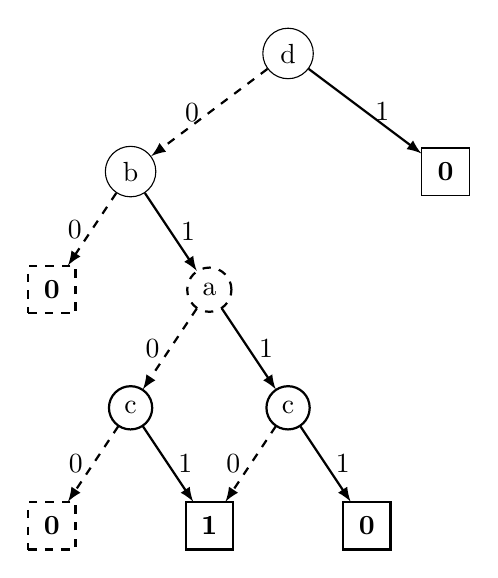
\begin{tikzpicture}[
        level distance=1.5cm,
        level 1/.style={sibling distance=4cm},
        level 2/.style={sibling distance=2cm},
        level 3/.style={sibling distance=2cm},
        solid edge/.style={solid, thick, -latex},
        dashed edge/.style={dashed, thick, -latex},
        terminal/.style={draw, rectangle, minimum size=0.6cm, font=\bfseries}
    ]
        % Root node d
        \node[circle, draw] {d}
            child { node[circle, draw] {b}
                child { node[terminal] {0}
                    edge from parent[dashed edge] node[left] {0}
                }
                child { node[circle, draw] {a}
                    child { node[circle, draw] {c}
                        child { node[terminal] {0} edge from parent[dashed edge] node[left] {0} }
                        child { node[terminal] {1} edge from parent[solid edge] node[right] {1} }
                        edge from parent[dashed edge] node[left] {0}
                    }
                    child { node[circle, draw] {c}
                        child { node[terminal] {1} edge from parent[dashed edge] node[left] {0} }
                        child { node[terminal] {0} edge from parent[solid edge] node[right] {1} }
                        edge from parent[solid edge] node[right] {1}
                    }
                    edge from parent[solid edge] node[right] {1}
                }
                edge from parent[dashed edge] node[left] {0}
            }
            child { node[terminal] {0}
                edge from parent[solid edge] node[right] {1}
            };
            
    \end{tikzpicture}
\end{figure}

% ==============================================================================
\section{Bài 8 (1đ): Tối ưu hóa Datapath}
\textbf{ĐỀ BÀI:} \\
Tối ưu thiết kế sau sử dụng các kỹ thuật:\\
- Chia sẻ tài nguyên, chia sẻ biểu thức chung\\
- Thay đổi, sắp xếp toán tử\\
- Tối ưu biểu thức logic\\
(a) Phương trình hệ thống: $F1 = (X0 \times X1) + (X2 \times X3)$, $F2 = (X2 \times X3) - (X4 \times X5)$\\
(b) Sơ đồ logic: 
Cổng 1: $\overline{A \cdot B}$, 
Cổng 2: $\overline{C + D}$, 
Cổng 3: $\overline{A + B}$, 
Cổng 4: $\overline{C \cdot D}$\\
$F1 = (\overline{A \cdot B}) + (\overline{C + D})$, 
$F2 = (\overline{A + B}) + (\overline{C \cdot D})$

\hrule\vspace{0.5cm}
\textbf{LỜI GIẢI:}

\textbf{Sơ đồ (a): Chia sẻ biểu thức chung (Common Sub-expression Sharing)}
\begin{itemize}
    \item Nhận thấy biểu thức $(X2 \times X3)$ xuất hiện ở cả $F1$ và $F2$.
    \item \textbf{Tối ưu:} Thay vì sử dụng 3 bộ nhân như thiết kế gốc, ta chỉ cần sử dụng 2 bộ nhân:
    \begin{itemize}
        \item Cụm 1: $M_1 = X0 \times X1$
        \item Cụm 2: $M_2 = X2 \times X3$ (sử dụng chung cho F1 và F2)
        \item Cụm 3: $M_3 = X4 \times X5$
        \item $F1 = M_1 + M_2$
        \item $F2 = M_2 - M_3$
    \end{itemize}
    \item \textbf{Kết quả:} Tiết kiệm được 1 khối Multiplier (Bộ nhân).
\end{itemize}

\textbf{Sơ đồ (b): Tối ưu biểu thức logic (Logic Optimization)}
Áp dụng định lý De Morgan:
\begin{itemize}
    \item $F1 = \overline{A \cdot B} + \overline{C + D} = (\overline{A} + \overline{B}) + (\overline{C} \cdot \overline{D})$
    \item $F2 = \overline{A + B} + \overline{C \cdot D} = (\overline{A} \cdot \overline{B}) + (\overline{C} + \overline{D})$
\end{itemize}
Hoặc có thể tối ưu ở mức cổng như sau để tận dụng các cổng có sẵn:
\begin{itemize}
    \item F1 gốc cần NAND, NOR, OR. F2 gốc cần NOR, NAND, OR.
    \item Có thể áp dụng chia sẻ cổng đảo (Inverters) cho tín hiệu A, B, C, D để tổng hợp mạch nhanh hơn và dùng chung các cổng AND, OR phía sau.
\end{itemize}

\end{document}
